\chapter{Funktionsweise}
Deferred-Shading ist eine Rendering Technik die den Shading-Vorgang, wie etwa die Beleuchtungsberechnung, im Screen-Space durchführt. Im Gegensatz zum klassischen Forward-Shading sind die Berechnungen unabhängig von der Szenenkomplexität und ermöglichen somit unter anderem aufendiger beleuchtete Bilder.

Beim Forward-Shading wird die Geometrie in den Vertex-Shader gegeben, Transformationen und ähnliches angewandt und anschließend an den Rasterizer weiter gereicht, der die Fragmente berechnet die die Geometrie ausmachen. Im nächsten Schritt erhält der Fragment-Shader diese Fragmente und verarbeitet sie um die tatsächliche Farbe des Fragments zu bestimmen. Erst am Ende dieser Operationen wird mit dem Tiefentest festgestellt, ob das berechenete Fragment auf dem Bildschirm angezeigt wird \ref{fig:forward}. Das hat zur Folge, dass das Shading einer Szene von der Komplexität der Geometrie in der Szene abhängig ist. Demnach ist eine Szenenbeleuchtung, mit einer großen Anzahl an Lichtquellen, mittels Forward-Shading sehr rechenaufwändig.


\begin{figure}
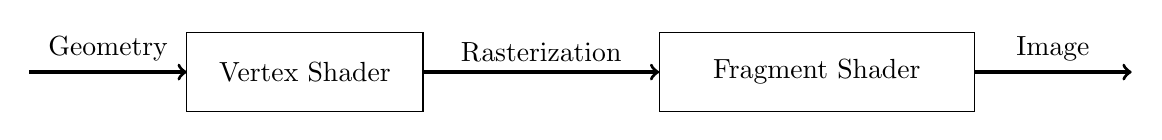
\begin{tikzpicture}
\draw[->, very thick] (0,0.5) -- (2, 0.5) node[pos=.5, above] {Geometry};
\draw (2,0) rectangle (5,1) node[pos=.5]{Vertex Shader};
\draw[->, very thick] (5,0.5) -- (8, 0.5) node[pos=.5, above] {Rasterization};
\draw (8,0) rectangle (12,1) node[pos=.5]{Fragment Shader};
\draw[->, very thick] (12,0.5) -- (14, 0.5) node[pos=.5, above] {Image};
\end{tikzpicture}
\caption{Forward-Rendering Pass}
\label{fig:forward}
\end{figure}

\footnote{Zur besseren Veranschaulichung wurde in obigem Diagramm auf die Operationen die nach Ausführung des Fragment-Shaders, sowie der Shading-Stages die zwischen Vertex- und Fragment-Shader liegen können, verzichtet}

Deferred-Shading ist ein Ansatz um dieses Problem zu lösen. Dabei wird der Render-Vorgang in zwei Schritte geteilt. Im ersten Schritt wird die Geometrie mit allen für die Beleuchtung benötigten Informationen, wie etwa der Frabe, der Normalen und Material-Eigenschaften, in einen Buffer gerendert \textendash{} den sog. Geometry-Buffer. Im zweiten Schritt wird nun die Beleuchtung, mithilfe des G-Buffers, im Screen-Space berechnet. Dazu wird ein Quadrat auf größe des Bildschirms gerendert, das das fertige Bild enthält \ref{fig:deferred}. An der Beleuchtungsberechnung selbst ändert sich beim Deferred-Shading nichts. Im zweiten Pass ist es nicht mehr möglich direkt an die Position der Vertices zu gelangen, allerdings lässt sich mithilfe des Depth-Buffers und den Fragmentkoordinaten im Screen-Space die frühere Position des Fragments innerhalb der Szene ermitteln. So wird Bandbreite und Speicher auf der Grafikkarte gespart, da die Fragementpositionen nicht mit im G-Buffer gespeichert werden müssen.


\begin{figure}
\begin{subfigure}[b]{0.5\textheight}
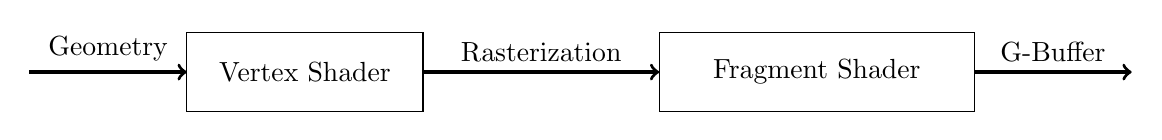
\begin{tikzpicture}
\draw[->, very thick] (0,0.5) -- (2, 0.5) node[pos=.5, above] {Geometry};
\draw (2,0) rectangle (5,1) node[pos=.5]{Vertex Shader};
\draw[->, very thick] (5,0.5) -- (8, 0.5) node[pos=.5, above] {Rasterization};
\draw (8,0) rectangle (12,1) node[pos=.5]{Fragment Shader};
\draw[->, very thick] (12,0.5) -- (14, 0.5) node[pos=.5, above] {G-Buffer};
\end{tikzpicture}
\caption{First Pass}
\end{subfigure}

\begin{subfigure}[b]{0.5\textheight}
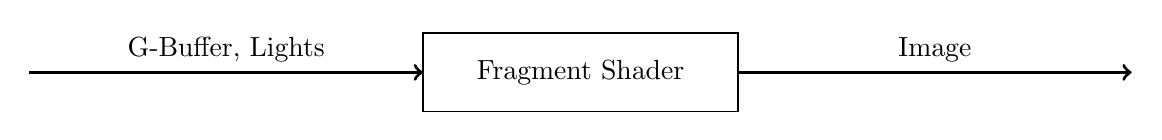
\begin{tikzpicture}
\draw[->, very thick] (0,4.5) -- (5, 4.5) node[pos=.5, above] {G-Buffer, Lights};
\draw (5,4) rectangle (9,5) node[pos=.5]{Fragment Shader};
\draw[->, very thick] (9,4.5) -- (14, 4.5) node[pos=.5, above] {Image};
\end{tikzpicture}
\caption{Second Pass}
\end{subfigure}
\caption{Deferred-Rendering Pass}
\label{fig:deferred}
\end{figure}
\footnote{Zur besseren Veranschaulichung wurden in der obigen Darstellung auf einige Schritte verzichtet}